Für diese Referenzarchitektur käme sowohl der Dienst der Multimode Klasse, \AWSIOT{} Analytics, als auch Timestream, als bester der Batch-Klasse in Frage. Da Timestream im Vergleich besser abschnitt, wird im Folgenden die Referenzarchitektur mit Timestream konstruiert.
Diese Referenzarchitektur entspricht dem in \autoref{chap:bestehende_ras} vorgestellten Konzept einer \ac{OLAP}-Architektur.

\subsection{Datenverarbeitungssequenz}

\begin{figure}[H]
\centering
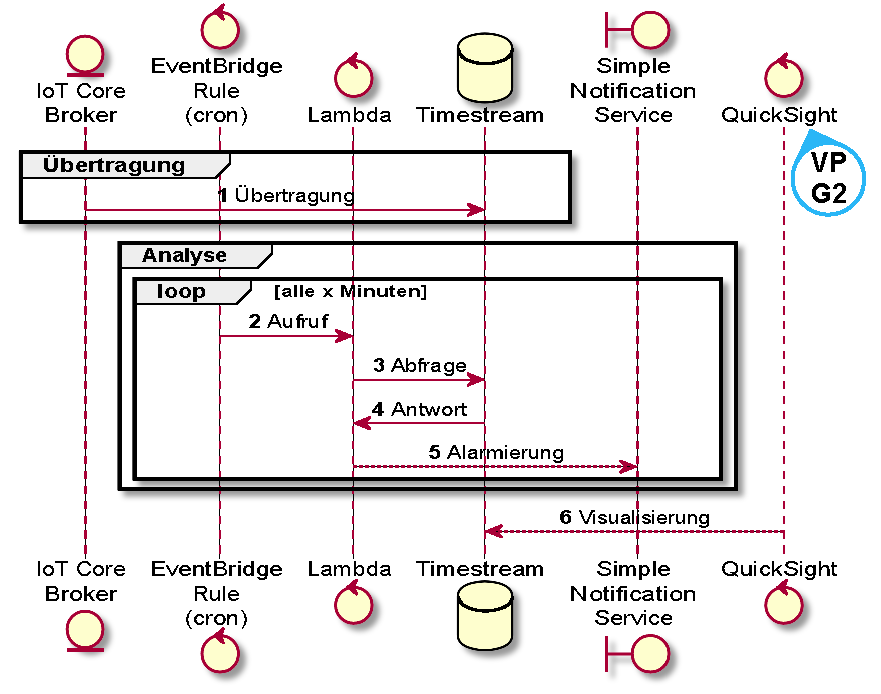
\includegraphics[width=\textwidth]{graphics/batch-ra.pdf}
\caption{Sequenzdiagramm Batch Verarbeitung}
\label{abb:SequenceBatchRA}
\end{figure}

\subsection{Verteilungssicht}
\begin{figure}[H]
\centering
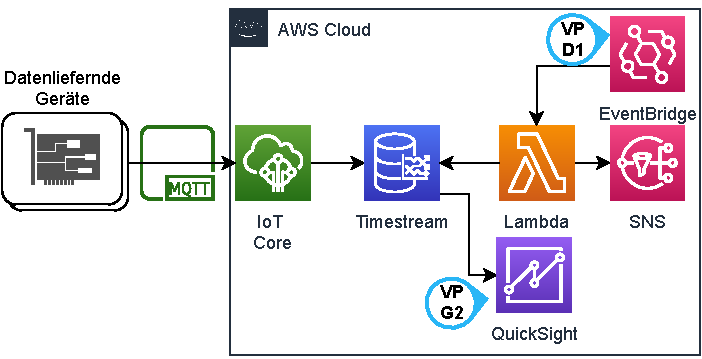
\includegraphics[width=\textwidth]{graphics/DB-RA-Overview.pdf}
\caption{Top Level View Referenzarchitektur}
\label{abb:TopLevelDBRA}
\end{figure}

\vp{D1}: Hier wird eine Dashboardinglösung, im speziellen der \ac{AWS} eigenen Dienst QuickSight eingeplant. Dies erfolgt, damit Benachrichtigungen, die via \ac{SNS} versendet werden, leicht für die Benachrichtigten nachvollziehbar sind. Wenn also beispielsweise eine Anomalie erkannt wurde, kann dies mit einer Visualisierung nachvollzogen werden, um dann entsprechend zu handeln. Wichtig ist, dass die Visualisierung sowohl von den Originaldaten aus dem Speicher von \AWSIOT{} Analytics gespeist wird, als auch aus der Analyse. Eine Visualisierung sieht wie folgt aus:

\textbf{Variationspunkt G2:} Siehe \vpref{G2}. Aber auch: native Integration mit Grafana/ Amazon Managed service for Grafana

\begin{figure}[H]
\centering
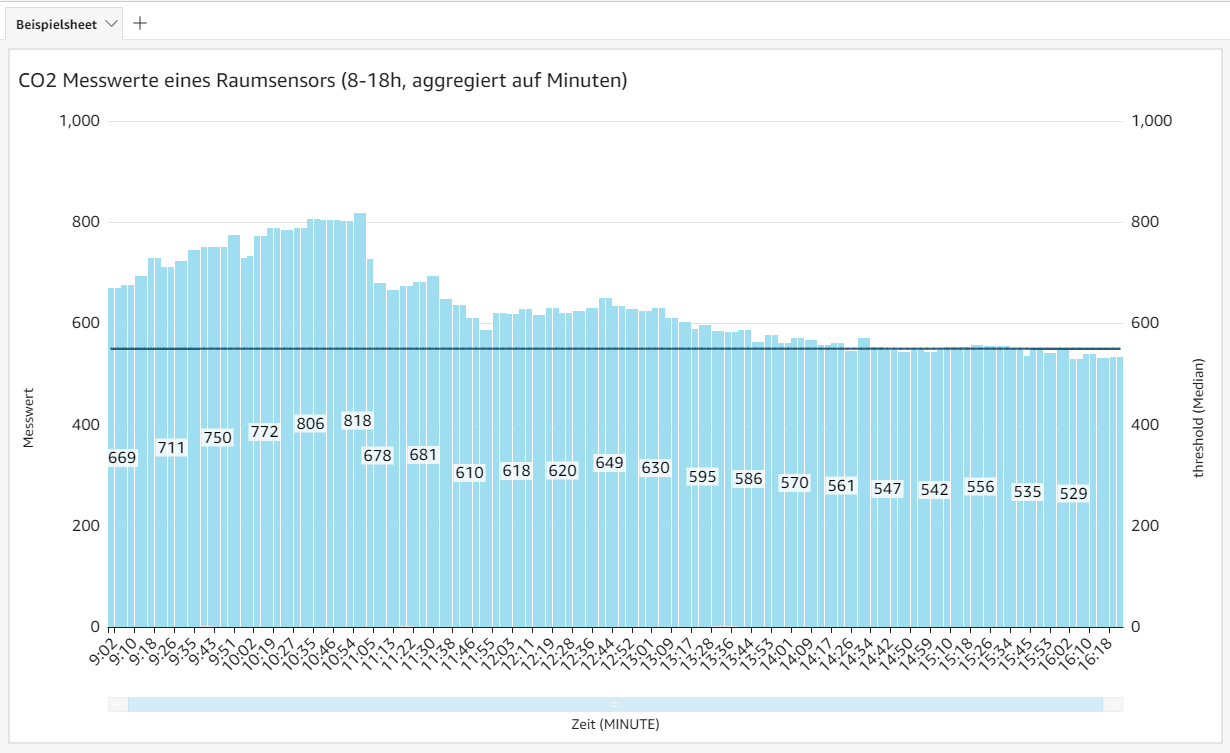
\includegraphics[width=\textwidth]{graphics/QuickSight-Beispiel.png}
\caption{Dashboard in Quicksight}
\label{abb:DashboardDBRA}
\end{figure}

Hier können Benachrichtigte direkt ablesen, dass ständige Schwellwert-Alarme am Morgen ihre Berechtigung hatten, da der Schwellwert erst gegen 14.30 Uhr unterschritten wurde. Entsprechend Maßnahmen, wie beispielsweise die gezielte Belüftung des Raums, in welchem dieser Sensor war, können eingeleitet werden.

\subsection{Bausteinsicht}
\begin{figure}[H]
\centering
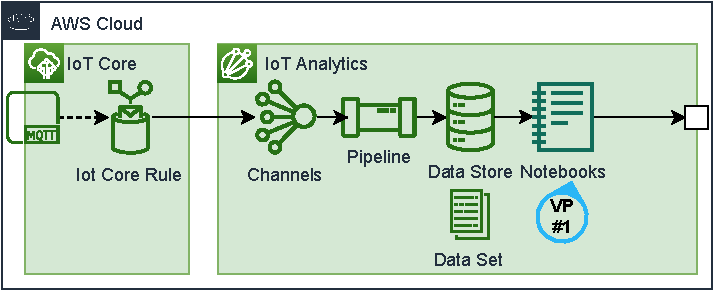
\includegraphics[width=\textwidth]{graphics/DB-RA-Elements.pdf}
\caption{Interagierende Dienstelemente}
\label{abb:ElementeDBRA}
\end{figure}

\vp{E1}:  Datenretention in Mem => Preis/Leistungsbalance

\vp{E2}: Selbst zu schreibende \ac{SQL}-Abfragen - Thema Queryoptimierung

\vp{E3}: Selbst zu schreibende Lambda Funktion siehe \anhangref{anhang:batch-codesample}

\vp{E4}: Custom Dashboards

\vp{E5}: Anpassen nach cron schedule oder fixierte Rate alle x Minuten, Stunden, Tage

\textbf{Variationspunkt G5}: Siehe \vpref{G5}

\subsection{Anforderungen}
\begin{itemize}
\item Anwendbarkeit auf Monitoringdaten (IT)
Funktioniert nicht mit Logs nur mit Metriken

\item Anwendbarkeit auf Sensordaten (\ac{IoT})

\item Wertschöpfung für das Unternehmen wichtig

\item akzeptabel und problemlösend für Domäne

\item Handling von Events, Messwerten und \enquote{Streaming}

Ingestionlatenz Beispiel

\item automatisierte operative Entscheidungen\\
Wie in \anhangref{anhang:batch-codesample} gezeigt möglich.
\end{itemize}

\subsection{Operations}

\begin{table}[H]
\centering
\begin{tabular}{|l|l|l|l|}
\hline
Dienst & Metrik & Ursache & Detektionsart \\ \hline
\rowcolor[HTML]{F5F5F5} 
\ac{SNS} & NumberOfNotificationsFailed & Dienstfehler & Schwellwert \\ \hline

\multirow{2}{*}{\AWSIOT{} Core} & RuleMessageThrottled & \begin{tabular}[c]{@{}l@{}}Dienstfehler/\\ Benutzungsfehler\end{tabular} & Schwellwert \\ \cline{2-4} 
 & Failure & \begin{tabular}[c]{@{}l@{}}Dienstfehler/\\ Benutzungsfehler\end{tabular} & Schwellwert \\ \hline
 
\rowcolor[HTML]{F5F5F5} 
\cellcolor[HTML]{F5F5F5} & SystemErrors & Dienstfehler & Schwellwert \\ \cline{2-4} 
\rowcolor[HTML]{F5F5F5} 
\cellcolor[HTML]{F5F5F5} & UserErrors & Benutzungsfehler & Schwellwert \\ \cline{2-4} 
\rowcolor[HTML]{F5F5F5} 
\multirow{-3}{*}{\cellcolor[HTML]{F5F5F5}TimeStream} & SuccessfulRequestLatency & \begin{tabular}[c]{@{}l@{}}Dienstfehler/\\ Benutzungsfehler\end{tabular} & Anomalie \\ \hline

\multirow{3}{*}{Lambda} & Duration & \begin{tabular}[c]{@{}l@{}}Dienstfehler/\\ Benutzungsfehler\end{tabular} & Anomalie \\ \cline{2-4} 
 & Errors & \begin{tabular}[c]{@{}l@{}}Dienstfehler/\\ Benutzungsfehler\end{tabular} & Schwellwert \\ \cline{2-4} 
 & Throttles & Benutzungsfehler & Schwellwert \\ \hline
 
\rowcolor[HTML]{F5F5F5} 
\multirow{2}{*}{EventBridge} & FailedInvocations & Dienstfehler & Anomalie \\ \cline{2-4} 
 & ThrottledRules & Dienstfehler & Schwellwert \\ \hline
 
 
\end{tabular}
\caption{CloudWatch Metriken}
\label{tab:cloudwatch-metrics-db}
\end{table}


TimeStream \footcite[Vgl.][]{AmazonWebServicesInc..o.J.be}
Lambda \footcite[Vgl.][]{AmazonWebServicesInc..o.J.bf}
\ac{SNS} \footcite[Vgl.][]{AmazonWebServicesInc..o.J.bc}
\AWSIOT{} Core \footcite[Vgl.][]{AmazonWebServicesInc..o.J.az}
EventBridge \footcite[Vgl.][]{AmazonWebServicesInc..o.J.bl}

\subsection{Know-how}
TimeStream nur in eu-west-1

Datenspeicherungsoptimierung

Datenspeicherung in Dimensionen und Attributen


\section{Einsatzszenarien der Referenzmodelle}


Chaos Engineering nicht vergessen \footcite[Vgl.][]{Augsten.2020}

Innerhalb dieser Arbeit wurden Referenzarchitekturen für die Verarbeitung in der Cloud konstruiert. Ein Trend, der dabei ausgespart wurde, ist das sogenannte \enquote{Fog computing}. Nach der Definition von \citeauthor{Vaquero.2014} ist Fog computing ein Szenario, in dem heterogene, allgegenwärtige und dezentralisierte Geräte kommunizieren und kooperieren um Speicher- und Verarbeitungsaufgaben zu übernehmen.\footcite[Vgl.][30\psq]{Vaquero.2014} In der Praxis führt dies dazu, dass Verarbeitungsaufgaben in Teilen, angelehnt an das \enquote{Edge computing} von der Cloud in Richtung der Geräte ausgelagert wird.\footcite[Vgl.][]{Bonomi.2012} Dies geschieht dabei beispielsweise an Netzwerkgateways, die sowieso mit der Cloud kommunizieren und folgend nur noch bereits ausgewertete Daten übertragen.

Gateways mit GreenGrass \footcite[][]{Shankar.2020}